
\documentclass{beamer}
\usepackage[utf8]{inputenc}

\usetheme{Madrid}
\usecolortheme{default}
\usepackage{amsmath,amssymb,amsfonts,amsthm}
\usepackage{txfonts}
\usepackage{tkz-euclide}
\usepackage{listings}
\usepackage{adjustbox}
\usepackage{array}
\usepackage{tabularx}
\usepackage{gvv}
\usepackage{lmodern}
\usepackage{circuitikz}
\usepackage{tikz}
\usepackage{graphicx}
\usepackage{gensymb}
\usepackage{enumitem}
\usepackage{etoolbox}
\setbeamertemplate{page number in head/foot}{}

\title{1.1.3 - Spring Mass Damper System}
\date{March 25, 2026}
\author{ADHARVAN KSHATHRIYA BOMMAGANI - EE25BTECH11003}

\begin{document}

\frame{\titlepage}

% Question
\begin{frame}{Question}
A spring-mass-damper system is excited by a force $F_0 \sin \omega t$. The amplitude at resonance is measured to be $1$ cm. At half the resonance frequency, the amplitude is $0.5$ cm. The damping ratio of the system is:

\begin{enumerate}[label=\alph*)]
    \item $0.1026$
    \item $0.3242$
    \item $0.7211$
    \item $0.1936$
\end{enumerate}
\end{frame}

% Step 1
\begin{frame}{Theoretical Solution}
From Newton's Second Law:
\[
m\ddot{x} + c\dot{x} + kx = F_0 \sin(\omega t)
\]

\begin{figure}
    \centering
    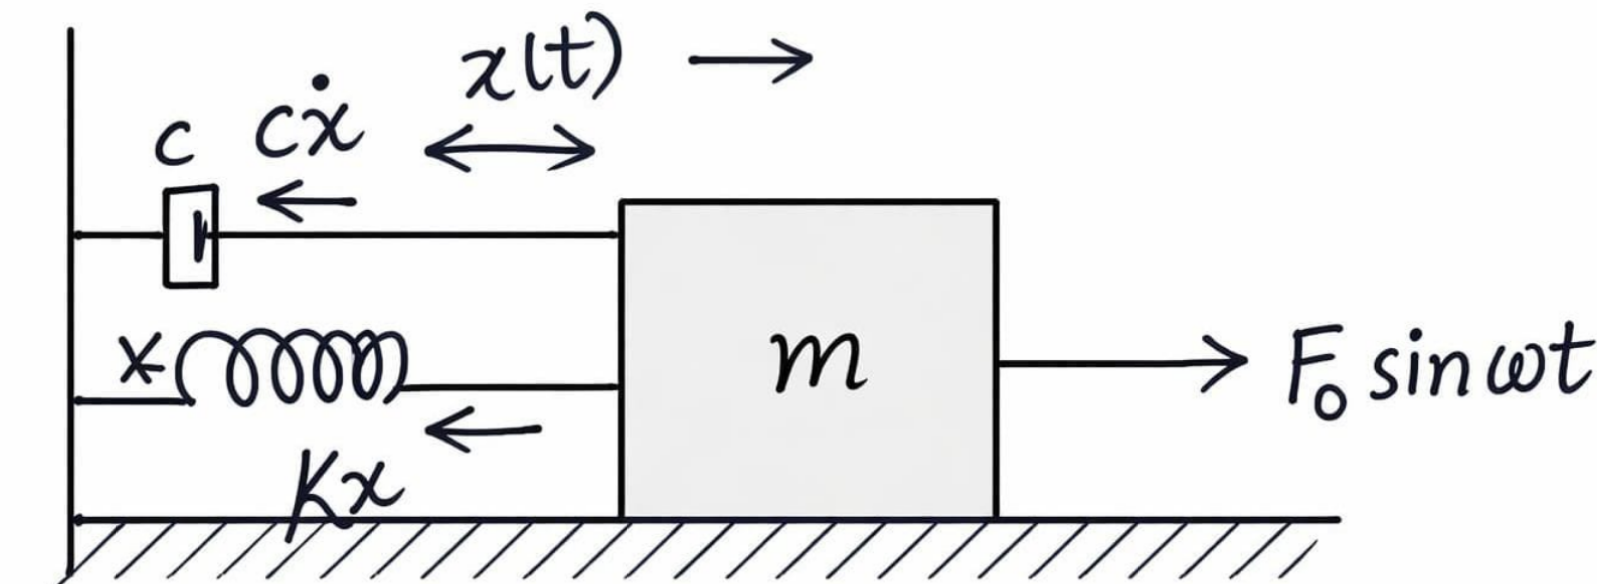
\includegraphics[width=0.5\linewidth]{image1.png}
    \caption{Spring Mass Damper System}
\end{figure}
\end{frame}



% Response split
\begin{frame}{System Response}

For a second-order differential equation, two functions $x_{1}(t)$ and $x_{2}(t)$ that are linearly
independent statisfy the DE.
\[
x(t) = x_h(t) + x_p(t)
\]

\begin{itemize}
    \item $x_h(t)$ → transient response(complementary solution)
    \item $x_p(t)$ → steady-state response(particular solution)
\end{itemize}
\end{frame}





% Step 1
\begin{frame}{Governing Equation}
Consider the homogeneous equation:
\begin{align}
m\ddot{x} + c\dot{x} + kx = 0
\end{align}
\end{frame}

% Step 2
\begin{frame}{Assumed Solution}
Assume an exponential solution:
\begin{align}
x(t) = e^{st}
\end{align}

Then:
\begin{align}
\dot{x} = s e^{st}, \quad \ddot{x} = s^2 e^{st}
\end{align}
\end{frame}

% Step 3
\begin{frame}{Characteristic Equation}
Substitute into the differential equation:
\begin{align}
ms^2 e^{st} + cs e^{st} + k e^{st} = 0
\end{align}

Divide by $e^{st}$:
\begin{align}
ms^2 + cs + k = 0
\end{align}
\end{frame}

% Step 4
\begin{frame}{Roots of Characteristic Equation}
\begin{align}
s = \frac{-c \pm \sqrt{c^2 - 4mk}}{2m}
\end{align}

Define:
\begin{align}
\omega_n = \sqrt{\frac{k}{m}}, \quad
\zeta = \frac{c}{2\sqrt{km}}
\end{align}
\end{frame}


% Step 6
\begin{frame}{General Solution}
\begin{align}
x_h(t) = C_1 x_{1}(t)
+ C_2 x_{2}(t)
\end{align}
\begin{align}
x_h(t) = C_1 e^{(-\zeta \omega_n + i\omega_d)t}
+ C_2 e^{(-\zeta \omega_n - i\omega_d)t}
\end{align}
\end{frame}

% Step 7
\begin{frame}{Convert to Real Form}
Factor:
\begin{align}
x_h(t) = e^{-\zeta \omega_n t}
\left(C_1 e^{i\omega_d t} + C_2 e^{-i\omega_d t}\right)
\end{align}

Using Euler’s formula:
\begin{align}
e^{i\theta} = \cos\theta + i\sin\theta
\end{align}
\end{frame}

% Step 8
\begin{frame}{Final Transient Response}
\begin{align}
x_h(t) = e^{-\zeta \omega_n t}
\left(A \cos \omega_d t + B \sin \omega_d t\right)
\end{align}
\end{frame}

% Interpretation
\begin{frame}{Physical Interpretation}
\begin{itemize}
    \item $e^{-\zeta \omega_n t}$ → exponential decay
    \item $\cos, \sin$ → oscillatory motion
    \item $\omega_d < \omega_n$ → reduced frequency due to damping
\end{itemize}
\end{frame}

% Physical meaning
\begin{frame}{Physical Meaning of Transient}
\begin{itemize}
    \item Caused by initial conditions
    \item Energy dissipates due to damping
\end{itemize}

\[
x(t) \sim e^{-\zeta \omega_n t}
\]

\begin{itemize}
    \item Eventually vanishes
\end{itemize}
\end{frame}


% Laplace
\begin{frame}{Laplace Transform}
\[
m s^2 X(s) + c s X(s) + k X(s) = \frac{F_0 \omega}{s^2 + \omega^2}
\]

\[
X(s) = \frac{F_0 \omega}{(s^2 + \omega^2)(ms^2 + cs + k)}
\]
\end{frame}







% Steady state
\begin{frame}{Steady-State Response}

For steady state response, $s= i\omega$,
\[
X(i\omega) = \frac{F_0}{k - m\omega^2 + i c\omega}
\]

\[
X = \frac{F_0}{\sqrt{(k - m\omega^2)^2 + (c\omega)^2}}
\]
\end{frame}

% Complete solution
\begin{frame}{Complete Solution}
\[
x(t) =
e^{-\zeta \omega_n t}(A\cos \omega_d t + B\sin \omega_d t)
+ X \sin(\omega t - \phi)
\]
\end{frame}

% Long time
\begin{frame}{Long-Time Behaviour}
As $t \to \infty$:
\[
e^{-\zeta \omega_n t} \to 0
\]

\[
x(t) \to X \sin(\omega t - \phi)
\]
\end{frame}

% Non dimensional
\begin{frame}{Non-Dimensional Form}
Define:
\begin{align}
\omega_n = \sqrt{\frac{k}{m}}, \quad
r = \frac{\omega}{\omega_n}, \quad
\zeta = \frac{c}{2\sqrt{km}}
\end{align}

\begin{align}
X = \frac{F_0/k}{\sqrt{(1 - r^2)^2 + (2\zeta r)^2}}
\end{align}
\end{frame}
% Apply conditions
\begin{frame}{Apply Conditions}

At resonance $r \approx 1$, As frequency of oscillation would be equal to natural frequency,
\[
X_{\text{res}} = \frac{F_0/k}{2\zeta} = 1
\]

\[
X_{0.5} = \frac{F_0/k}{\sqrt{0.75^2 + \zeta^2}} = 0.5
\]
\end{frame}

% Solve
\begin{frame}{Solve}
\[
\frac{2\zeta}{\sqrt{0.75^2 + \zeta^2}} = 0.5
\]

\[
\zeta = 0.1936
\]
\end{frame}

% Final
\begin{frame}{Final Answer}
\[
\boxed{\zeta = 0.1936}
\]

\begin{itemize}
    \item Correct option: \textbf{(d)}
\end{itemize}
\end{frame}

\begin{frame}[fragile]{Python Plot: Displacement vs Time}
\begin{lstlisting}
import numpy as np
import matplotlib.pyplot as plt
# System parameters
zeta = 0.1936
omega_n = 1.0
omega = omega_n
# Derived quantities
omega_d = omega_n * np.sqrt(1 - zeta**2)
# Constants
A = 1.0
B = 0.0
# Steady-state amplitude
X = 1 / (2 * zeta)

\end{lstlisting}
\end{frame}
\begin{frame}[fragile]{Python Plot: Displacement vs Time}
\begin{lstlisting}
# Phase at resonance
phi = np.pi / 2
# Time range (increased)
t = np.linspace(0, 150, 4000)
# Transient response
x_h = np.exp(-zeta * omega_n * t) * \
      (A*np.cos(omega_d*t) + B*np.sin(omega_d*t))

# Steady-state response
x_p = X * np.sin(omega * t - phi)
# Total response
x = x_h + x_p
# Plot
plt.plot(t, x, label="Total")
plt.plot(t, x_h, '--', label="Transient")
plt.plot(t, x_p, ':', label="Steady-State")
\end{lstlisting}
\end{frame}
\begin{frame}[fragile]{Python Plot: Displacement vs Time}
\begin{lstlisting}
plt.xlabel("Time")
plt.ylabel("Displacement")
plt.title("Transient to Steady-State Response")
plt.legend()
plt.grid()
plt.show()
\end{lstlisting}
\end{frame}

\begin{frame}{Plot}
    
\begin{figure}
    \centering
    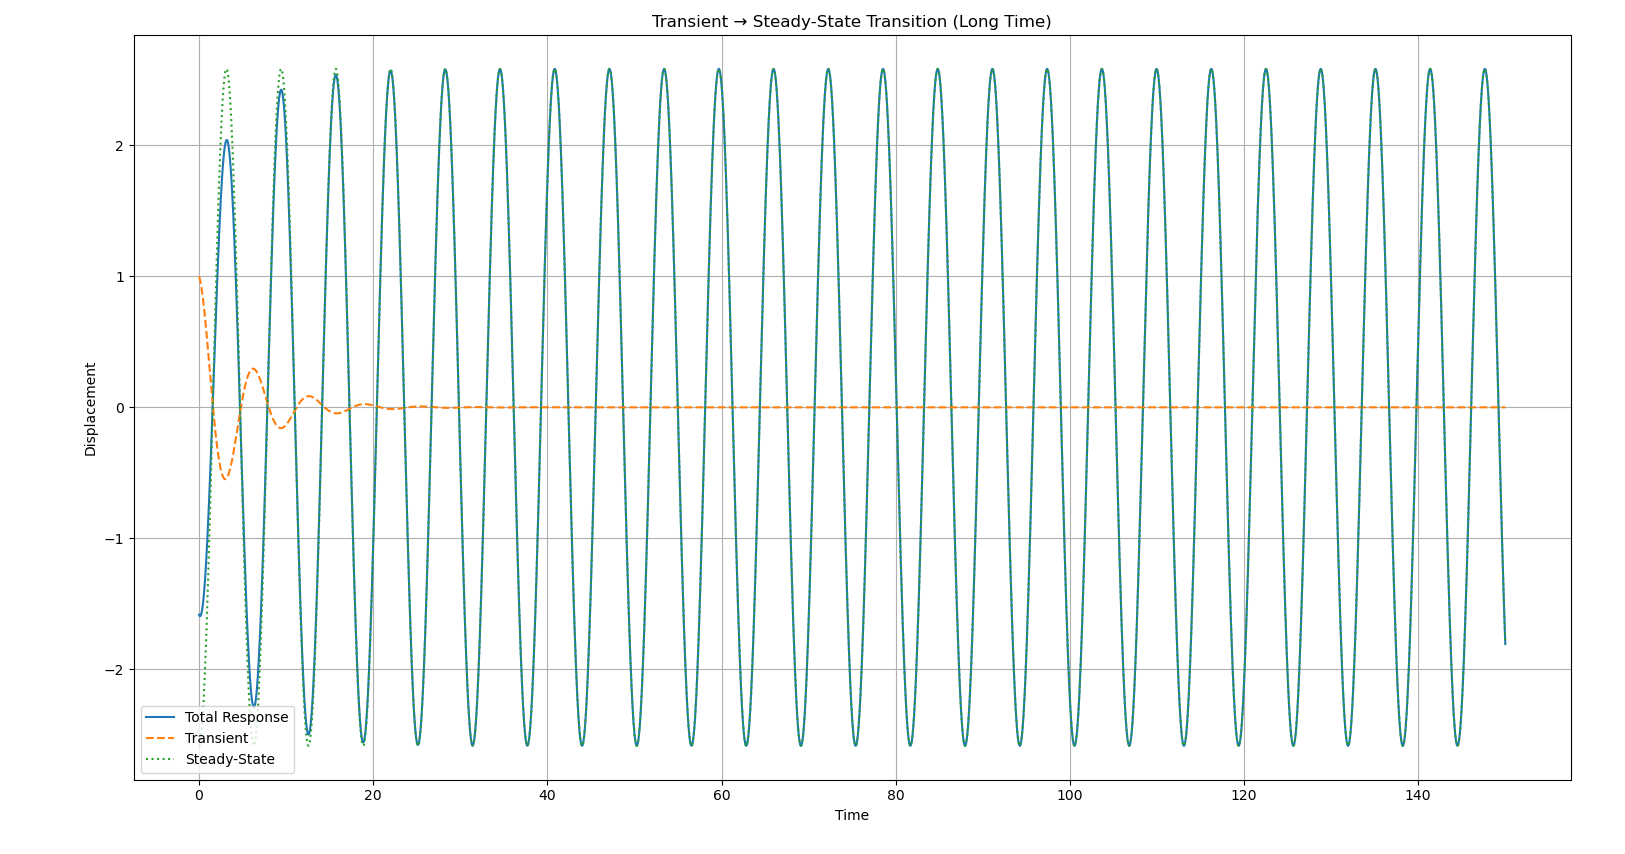
\includegraphics[width=0.75\linewidth]{image2.png}
    \caption{Plot of Displacement versus Time}
\end{figure}
\end{frame}

\end{document}
